\documentclass[floatsintext,man]{apa6}

\usepackage{amssymb,amsmath}
\usepackage{ifxetex,ifluatex}
\usepackage{fixltx2e} % provides \textsubscript
\ifnum 0\ifxetex 1\fi\ifluatex 1\fi=0 % if pdftex
  \usepackage[T1]{fontenc}
  \usepackage[utf8]{inputenc}
\else % if luatex or xelatex
  \ifxetex
    \usepackage{mathspec}
    \usepackage{xltxtra,xunicode}
  \else
    \usepackage{fontspec}
  \fi
  \defaultfontfeatures{Mapping=tex-text,Scale=MatchLowercase}
  \newcommand{\euro}{€}
\fi
% use upquote if available, for straight quotes in verbatim environments
\IfFileExists{upquote.sty}{\usepackage{upquote}}{}
% use microtype if available
\IfFileExists{microtype.sty}{\usepackage{microtype}}{}

% Table formatting
\usepackage{longtable, booktabs}
\usepackage{lscape}
% \usepackage[counterclockwise]{rotating}   % Landscape page setup for large tables
\usepackage{multirow}		% Table styling
\usepackage{tabularx}		% Control Column width
\usepackage[flushleft]{threeparttable}	% Allows for three part tables with a specified notes section
\usepackage{threeparttablex}            % Lets threeparttable work with longtable

% Create new environments so endfloat can handle them
% \newenvironment{ltable}
%   {\begin{landscape}\begin{center}\begin{threeparttable}}
%   {\end{threeparttable}\end{center}\end{landscape}}

\newenvironment{lltable}
  {\begin{landscape}\begin{center}\begin{ThreePartTable}}
  {\end{ThreePartTable}\end{center}\end{landscape}}




% The following enables adjusting longtable caption width to table width
% Solution found at http://golatex.de/longtable-mit-caption-so-breit-wie-die-tabelle-t15767.html
\makeatletter
\newcommand\LastLTentrywidth{1em}
\newlength\longtablewidth
\setlength{\longtablewidth}{1in}
\newcommand\getlongtablewidth{%
 \begingroup
  \ifcsname LT@\roman{LT@tables}\endcsname
  \global\longtablewidth=0pt
  \renewcommand\LT@entry[2]{\global\advance\longtablewidth by ##2\relax\gdef\LastLTentrywidth{##2}}%
  \@nameuse{LT@\roman{LT@tables}}%
  \fi
\endgroup}


  \usepackage{graphicx}
  \makeatletter
  \def\maxwidth{\ifdim\Gin@nat@width>\linewidth\linewidth\else\Gin@nat@width\fi}
  \def\maxheight{\ifdim\Gin@nat@height>\textheight\textheight\else\Gin@nat@height\fi}
  \makeatother
  % Scale images if necessary, so that they will not overflow the page
  % margins by default, and it is still possible to overwrite the defaults
  % using explicit options in \includegraphics[width, height, ...]{}
  \setkeys{Gin}{width=\maxwidth,height=\maxheight,keepaspectratio}
\ifxetex
  \usepackage[setpagesize=false, % page size defined by xetex
              unicode=false, % unicode breaks when used with xetex
              xetex]{hyperref}
\else
  \usepackage[unicode=true]{hyperref}
\fi
\hypersetup{breaklinks=true,
            pdfauthor={},
            pdftitle={Child language experience in a Tseltal Mayan village},
            colorlinks=true,
            citecolor=blue,
            urlcolor=blue,
            linkcolor=black,
            pdfborder={0 0 0}}
\urlstyle{same}  % don't use monospace font for urls

\setlength{\parindent}{0pt}
%\setlength{\parskip}{0pt plus 0pt minus 0pt}

\setlength{\emergencystretch}{3em}  % prevent overfull lines


% Manuscript styling
\captionsetup{font=singlespacing,justification=justified}
\usepackage{csquotes}
\usepackage{upgreek}

 % Line numbering
  \usepackage{lineno}
  \linenumbers


\usepackage{tikz} % Variable definition to generate author note

% fix for \tightlist problem in pandoc 1.14
\providecommand{\tightlist}{%
  \setlength{\itemsep}{0pt}\setlength{\parskip}{0pt}}

% Essential manuscript parts
  \title{Child language experience in a Tseltal Mayan village}

  \shorttitle{Child language experience in a Tseltal Mayan village}


  \author{Marisa Casillas\textsuperscript{1}, Penelope Brown\textsuperscript{1}, \& Stephen C. Levinson\textsuperscript{1}}

  % \def\affdep{{"", "", ""}}%
  % \def\affcity{{"", "", ""}}%

  \affiliation{
    \vspace{0.5cm}
          \textsuperscript{1} Max Planck Institute for Psycholinguistics  }

  \authornote{
    Correspondence concerning this article should be addressed to Marisa
    Casillas, P.O. Box 310, 6500 AH Nijmegen, The Netherlands. E-mail:
    \href{mailto:Marisa.Casillas@mpi.nl}{\nolinkurl{Marisa.Casillas@mpi.nl}}
  }


  \abstract{Enter abstract here. Each new line herein must be indented, like this
line.}
  \keywords{Child-directed speech, Linguistic input, Non-WEIRD, Vocal maturity, Turn
taking \\

    \indent Word count: X
  }





\usepackage{amsthm}
\newtheorem{theorem}{Theorem}[section]
\newtheorem{lemma}{Lemma}[section]
\theoremstyle{definition}
\newtheorem{definition}{Definition}[section]
\newtheorem{corollary}{Corollary}[section]
\newtheorem{proposition}{Proposition}[section]
\theoremstyle{definition}
\newtheorem{example}{Example}[section]
\theoremstyle{definition}
\newtheorem{exercise}{Exercise}[section]
\theoremstyle{remark}
\newtheorem*{remark}{Remark}
\newtheorem*{solution}{Solution}
\begin{document}

\maketitle

\setcounter{secnumdepth}{0}



\section{Introduction}\label{intro}

A great deal of work in developmental language science revolves around
one central question: What linguistic evidence (i.e., what types and how
much) is needed to support first language acquisition? In pursuing this
topic, many researchers have fixed their sights on child-directed speech
(CDS), showing that it is linguistically distinctive
(REFS)\textbf{{[}TASK 00: Add missing references{]}}, interactionally
rich (REFS), preferred by infants (REFS), and---perhaps most
importantly---facilitates word learning (REFS). By all appearances, CDS
is an essential component for acquiring a first language. Yet
ethnographic reports from a number of traditional, non-Western
communities suggest that children easily acquire their community's
language(s) with little or no CDS (REFS). If so, CDS may not be
essential for learning language; just useful for facilitating certain
aspects of language development. In this paper we investigate the
language environment and early development of 10 Tseltal Mayan children
growing up in a community where past research has suggested that
caregivers use little CDS with infants and young children (REFS Brown).

\subsection{Child-directed speech}\label{intro-cds}

The amount of CDS children hear influences their language development,
particularly their vocabulary (REFS). For example, \textbf{{[}TASK 01:
Add examples of input-vocab link{]}}. CDS has also been linked to young
children's speed of lexical retrieval (REFS Weisleder; LuCiD) and
syntactic development (REFS Huttenlocher). \textbf{{[}TASK 02: Read
Huttenlocher and add details here{]}}. The conclusion drawn from much of
this work is that CDS is an ideal register for learning
words---especially concrete nouns and verbs---because it is tailored to
maximize a child's moment-to-moment interest and understanding (REFS).
Indeed, even outside of first-person interaction, infants and young
children prefer listening to CDS over adult-directed speech (REFS
ManyBabies, etc.), suggesting that CDS is useful in catching,
maintaining, and focusing children's attention. There are, however, a
few significant caveats to the body of work relating CDS quantity to
language development.

First, while there is overwhelming evidence linking CDS quantity to
vocabulary size, links to grammatical development are more scant (REFS:
Huttenlocher; Frank et al.). While the advantage of CDS for referential
word learning is clear, it is less obvious how CDS facilitates syntactic
learning. \textbf{{[}TASK 03: Add argument from Yurovsky paper +
refrences therein{]}} On the other hand, there is a wealth of evidence
that both children and adults' syntactic knowledge is highly lexically
specified (REFS), and that, crosslinguistically, children's vocabulary
size is one of the most robust predictors of their early syntactic
development (REFS). In short, what is good for the lexicon may also be
good for syntax. For now, however, the link between CDS and other
aspects of grammatical development still needs to be more thoroughly
tested.

A second caveat is that most work on CDS quantity uses summary measures
that average over the ebb and flow of interaction (e.g., proportion
CDS). In both child and adult interactions, verbal behaviors are highly
structured: while some occur at fairly regular intervals
(\enquote{periodic}), others occur in shorter, more intense bouts
separated by long periods of inactivity (\enquote{bursty} REFS Abney
2018 bursts and lulls, see also fusaroli et al. 2014 synergy). For
example, Abney and colleagues (2016 REFS) found that, across multiple
time scales of daylong recordings, both infants' and adults' vocal
behavior was clustered. Focusing on lexical development, Blasi and
colleagues (REFS in prep) also found that nouns and verbs were used
burstily in child-proximal speech across all six of the languages in
their typologically diverse sample. Infrequent words were somewhat more
bursty overall, leading them to propose that burstiness may play a key
and universal role in acquiring otherwise-rare linguistic units (see
also REFS in prep from
ICIS).\footnote{But see Drew and Bergelson (REFS in preparation), who find that the highest-frequency nouns used in CDS and children's own speech were relatively more bursty than other nouns.}
Experiment-based work also shows that two-year-olds learn novel words
better from a massed presentation of object labels versus a distributed
presentation (Schwab and Lew-Williams (2016) REFS; but see REFS Ambridge
et al., 2006; Childers and Tomasello, 2002). Structured temporal
characteristics in children's language experience imply new roles for
attention and memory in language development. By that token, we should
begin to investigate the link between CDS and linguistic development
with more nuanced measures of how CDS is distributed.

Finally, prior work has typically focused on Western (primarily North
American) populations, limiting our ability to generalize these effects
to children acquiring language worldwide (REFS: WEIRD; Lieven, 1994).
While we do gain valuable insight by looking at \emph{within-population}
variation (e.g., REFS), we can more effectively find places where our
assumptions break down by studying \emph{new} populations. Linguistic
anthropologists working in non-Western communities have long reported
that caregiver interaction styles vary immensely from place to place,
with some caregivers using little or no CDS to young children (REFS
Gaskins, 2006). Children in these communities reportedly acquire
language with \enquote{typical}-looking benchmarks. For example, they
start pointing (REFS Liszkowski et al., 2012; but see Salomo \&
Liszkowski, 2013) and talking (REFS Rogoff et al., 2003?; Brown??)
around the same time we would expect for Western middle-class infants.
These findings have had little impact on mainstream theories of word
learning and language acquisition, partly due to a lack of directly
comparable measures (Brown, 2014). If, however, these children indeed
acquire language without delay despite little or no CDS, we must
reconsider what kind of linguistic evidence is necessary for children to
learn language.

\subsection{Language development in non-WEIRD
communities}\label{intro-nonweird}

To our knowledge, only a handful of researchers have used methods from
developmental psycholinguistics to describe the language environments
and linguistic development of children growing up in traditional,
non-Western communities. We briefly highlight two recent efforts along
these lines, but see Mastin and Vogt (REFS 2016) and Cristia et al.
(2017) for more examples.

Scaff, Cristia, and colleagues (REFS 2017; in preparation) have used a
number of methods to estimate how much speech children hear in a Tsimane
forager-horticulturalist population in the Bolivian lowlands. Their
daylong recordings show that Tsimane children between 0;6 and 6;0 hear
\textasciitilde{}5 minutes of CDS per hour, regardless of their age (but
see Cristia et al., 2017). For comparison, children from North American
homes between ages 0;3 and 3;0 are estimated to hear \textasciitilde{}11
minutes of CDS per hour in daylong recordings (REFS: Bergelson,
Casillas, et al., see also REFS the newer Tamis-LeMonda paper; maybe
give estimates w/ age ranges for each??). Tsimane children also hear
\textasciitilde{}10 minutes of other-directed speech per hour (e.g.,
talk between adults) compared to the \textasciitilde{}7 minutes per hour
heard by North American children (REFS Bergelson, Casillas, et al.).
This difference may be attributable to the fact that the Tsimane live in
extended family clusters of 3--4 households, so speakers are typically
in close proximity to 5--8 other people (REFS Cristia et al., 2017).

Laura Shneidman and colleagues (REFS; 2010; 2012) analyzed speech from
1-hour at-home video recordings of children between ages 1;0 and 3;0 in
two communities: Yucatec Mayan (Southern Mexico) and North American (a
major U.S. city). Their analyses yielded four main findings: compared to
the American children, (a) the Yucatec children heard many fewer
utterances per hour, (b) a much smaller proportion of the utterances
they heard were \emph{child-directed}, (c) the proportion of utterances
that were child-directed increased dramatically with age, matching U.S.
children's by 3;0 months, and (d) most of the added CDS came from other
children (e.g., older siblings and cousins). They also demonstrated that
the lexical diversity of the CDS they hear at 24 months---particularly
from adult speakers---predicted children's vocabulary knowledge at 35
months.

These groundbreaking studies establish a number of important findings:
First, children in each of these communities appear able to acquire
their languages with relatively little CDS. Second, CDS might become
more frequent as children get older, though this could largely be due to
speech from other children. Finally, despite these differences, CDS from
adults may still be the most robust predictor of vocabulary growth.

\subsection{The current study}\label{intro-currentstudy}

We examine the early language experience of 10 Tseltal Mayan children
under age 3;0. Prior ethnographic work suggests that Tseltal caregivers
do not frequently speak directly to their children until the children
themselves begin speaking (REFS: Brown??). Nonetheless, Tseltal children
develop language with no apparent delays. Tseltal Mayan language and
culture has much in common with the Yucatec Mayan communities Shneidman
reports on (REFS: 2010 + add other stuff that's not nec lg), allowing us
to compare differences in child language environments between the two
sites more directly than before.\textbackslash{}footnote\{For a review
of comparative work on language socialization in Mayan cultures, see Pye
(2017).) We provide more details on this community and dataset in the
\protect\hyperlink{methods}{Methods section}.

Similar to previous work, we estimated how much speech children
overheard, how much was directed to them, and how those quantities
changed with age. To this foundation we added new sampling techniques
for investigating variability in children's speech environments within
daylong recordings. We also analyzed children's early vocal productions,
examining both the overall developmental trajectory of their vocal
maturity and how their vocalizations are influenced by CDS.

Based on prior work, we predicted that Tseltal Mayan children hear
little CDS, that the amount of CDS they hear increases with age, that
most CDS comes from other children, and that, despite this, Tseltal
Mayan children reach speech production benchmarks on par with Western
children. We additionally predicted that children's language
environments would be bursty---that brief, high-intensity interactions
would be sparsely distributed throughout the day, accounting for the
majority of children's daily CDS---and that children's responsiveness
and vocal maturity would be maximized during these moments of
high-intensity interaction.

\hypertarget{methods}{\section{Methods}\label{methods}}

\subsection{Community}\label{methods-community}

The children in our dataset (REFS: Casillas HomeBank) come from a
small-scale, subsistence farming community in the highlands of Chiapas
in Southern Mexico. The vast majority of children grow up speaking
Tseltal monolingually at home. Primary school is conducted in Tseltal,
but secondary and further education is primarily conducted in Spanish.
Nuclear families are often large (5+ children) and live in patrilineal
clusters. Nearly all families grow staple crops such as corn and beans,
but also bananas, chilies, squash, coffee, and more. Household and
farming work is divided among men, women, and older children. Women do
much of the daily cleaning and food preparation, but also frequently
work in the garden, haul water and firewood, and do other physical
labor. A few community members---both men and women---earn incomes as
teachers and shopkeepers but are still expected to regularly contribute
to their family's household work.

More than forty years of ethnographic work by the second author has
reported that Tseltal children's language environments are
non-child-centered and non-object-centered (REFS). During their waking
hours, Tseltal infants are typically tied to their mother's back while
she goes about her work for the day. Infants receive very little direct
speech until they themselves begin to initiate interactions, usually as
they approach their first birthdays. Even then, interactional exchanges
are often brief or non-verbal (e.g., object exchange routines) and take
place within a multi-participant context (Brown 2011; 2014). Rarely is
attention given to words and their meanings, even when objects are
central to the activity. Instead, interactions tend to focus on
appropriate actions and responses, and young children are socialized to
attend to the interactions taking place around them (REFS see also
Rogoff and de Leon).

Young children are often cared for by other family members, especially
older siblings. Even when not on their mother's back, infants are rarely
put on the ground, so they can't usually pick up the objects around them
until they are old enough to walk. Toys are scarce and books are
vanishingly rare, so the objects children do get their hands on tend to
be natural or household objects (e.g., rocks, sticks, spoons, baskets,
etc.). By age five, most children are competent speakers who engage
daily in chores and caregiving of their younger siblings. The Tseltal
approach to caregiving is similar to that described for other Mayan
communities (e.g., REFS Rogoff, Gaskins, de Leon, Shneidman).

\subsection{Corpus}\label{methods-corpus}

The current data come from the Casillas HomeBank Corpus (REFS HomeBank),
which includes daylong recordings and other developmental language data
from more than 100 children under 4;0 across two indigenous, non-WEIRD
communities: the Tseltal Mayan community described here and a Papua New
Guinean community described elsewhere (REFS).

\emph{{[}TASK 06: Check these demographic data again{]}} The Tseltal
data, primarily collected in 2015, include recordings from 55 children
born to 43 mothers. The families in our dataset typically only had 2--3
children (median = 2; range = 1--9), due to the fact that the
participating families come from a young subsample of the community
(mothers: mean = 26.9 years; median = 25.9; range = 16.6--43.8 and
fathers: mean = 30.5; median = 27.6; range = 17.7---52.9). On average,
mothers were 20.1 years old when they had their first child (median =
19; range = 12--27), with a following inter-child interval of 3.04 years
(median = 2.8; range =
1--8.5).\footnote{These estimates do not include miscarriages and/or children who passed away.}.
As a result, 26\% of the participating families had two children under
4;0.

Extended households, defined in our dataset as the group sharing a
kitchen or other primary living space, ranged between between 3 and 15
people (mean = NN; median = NN). Although 30.9\% of the target children
are first-born, they were rarely the only child in their extended
household. Caregiver education is one (imperfect) measure of contact
with Western culture. Most mothers had finished primary school, with
many also having completed secondary school (range = no
schooling--university). Most fathers had finished secondary school, with
many having also completed preparatory school (range = no
schooling--university). Owing in large part to patrilineal (i.e., father
to son) land inheritance, 93\% of the fathers grew up in the village
where the recordings took place, while only 53\% of the mothers did.

\subsubsection{Recordings}\label{methods-corpus-recs}

Methods for estimating the quantity of speech that children hear have
advanced significantly in the past two decades, with long-format at-home
audio recordings quickly becoming the new standard (e.g., with the
LENA\textsuperscript{®} system; REFS). These recordings capture a wider
range of the linguistic patterns children hear as they participate in
different activities with different speakers over the course of their
day. In longer, more naturalistic recordings, caregivers also tend to
use less CDS (REFS Tamis-LeMonda). The result is greater confidence that
the estimated CDS characteristics are representative of what the child
typically hears at home.

We used a novel combination of a lightweight stereo audio recorder
(Olympus\textsuperscript{®} WS-832) and wearable photo camera (Narrative
Clip 1\textsuperscript{®}) fitted with a fish-eye lens, to track
children's movements and interactions over the course of a 9--11-hour
period in which the experimenter was not present. Each recording was
made during a single day at home in which the recorder and/or camera was
attached to the child. Ambulatory children wore both devices on an
elastic vest. Non-ambulatory children wore the recorder in a onesie
while their primary caregiver wore the camera on an elastic vest
\emph{Figure 1} \emph{{[}TASK 07: Make figure{]}}. The camera was set to
take photos at 30-second intervals and was synchronized to the audio in
post-processing to create video of the child's daylong
recording.\footnote{Documentation for recording set-up and scripts for post-processing are available at *[TASK 08: Link to relevant docs]*}

\subsection{Data selection and annotation}\label{methods-samples}

We annotated video clips from 10 of the 55 children's recordings. We
chose these 10 recordings to maximize variance in three demographic
variables: child age (0--3;0), child sex, and maternal education. The
sample is summarized in \emph{Table 1} \emph{{[}TASK 09: Make table{]}}.
We then selected one hour's worth of non-overlapping clips from each
recording in the following order: nine randomly selected 5-minute clips,
five 1-minute clips manually selected as the top \enquote{turn-taking}
minutes of the recording, five 1-minute clips manually selected as the
top \enquote{vocal activity} minutes of the recording, and one, manually
selected 5-minute extension of the best 1-minute sample \emph{FIGURE ??}
\emph{{[}TASK 10: Add figure of recording times with samples highlighted
for the 10 recs{]}}. We created these different subsamples of each day
to measure properties of (a) children's \emph{average} language
environments (random samples) and (b) their \emph{most input-dense}
language environments (turn-taking samples). The third sample
(high-activity) gave us insight into children's productive speech
abilities.

The turn-taking and high-activity clips were chosen by two trained
annotators (the first author and a student assistant) who listened to
each recording in its entirety at 1--2x speed while actively taking
notes about potentially useful clips. Afterwards, the first author
reviewed the list of candidate clips, listened again to each one (at 1x
speed, multiple repetitions), and chose the best five 1-minute samples
for each of the two types of activity. Good turn-taking activity was
defined as at closely timed sequences of contingent vocalization between
the target child and at least one other person (i.e., frequent
vocalization exchanges). The \enquote{best} turn-taking clips were
chosen because they had the most and most clear turn-switching activity
between the target child and the other speaker(s). Good vocal activity
clips were defined as clips in which the target child produced the most
and most diverse spontaneous (i.e., not imitative) vocalizations. The
\enquote{best} vocal activity clips were chosen for representing the
most linguistically mature and/or diverse vocalizations made by the
child over the day. All else being equal, candidate clips were
prioritized when they contained less background noise or featured
speakers and speech that were not otherwise frequently represented
(e.g., CDS from older males). The best turn-taking clips and vocal
activity clips often overlapped; turn-taking clips were selected from
the list of candidates first, and then vocal-activity clips were chosen
from the remainder.

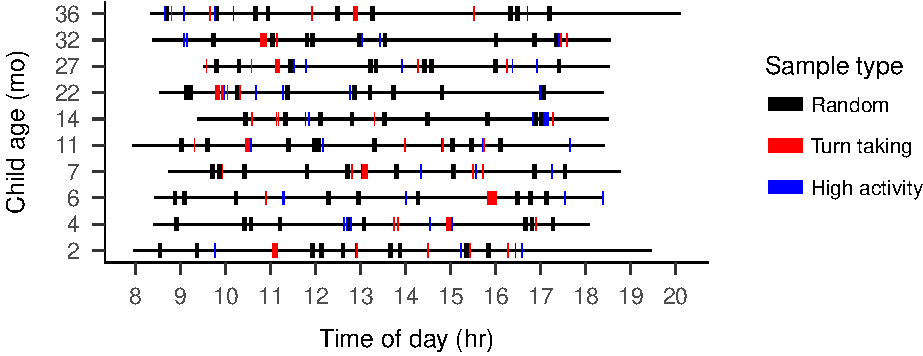
\includegraphics{Tseltal-CLE_files/figure-latex/fig0-1.pdf} Each video
clip was transcribed and annotated in ELAN (REFS) using the ACLEW
Annotation Scheme (REFS) by the first author and a native speaker of
Tseltal who lives in the community and knows most of the recorded
families personally. At the time of writing, NN\% \emph{{[}TASK XX: Fill
in before submitting{]}} of the clips have been reviewed by a second
native Tseltal speaker. The annotations include the transcription of
(nearly) all hearable utterances in Tseltal, a loose translation of each
utterance into Spanish, vocal maturity measures of each target child
utterance (non-linguistic vocalizations/non-canonical babbling/non-word
canonical babbling/single words/multiple words), and addressee
annotations for all non-target-child utterances
(target-child-directed/other-child-directed/adult-directed/adult-and-child-directed/animal-directed/other-speaker-type-directed).\footnote{Full documentation, including training materials, for the ACLEW Annotation Scheme can be found at *[TASK 11: Add OSF link]*.}

\subsubsection{Why vocal maturity?}\label{why-vocal-maturity}

\emph{{[}TASK 12: Missing paragraph!!{]}}

\subsection{Data analysis}\label{methods-analysisinfo}

We exported each ELAN file as tab-separated values and then the
annotations into R version 3.5.0 (2018-04-23) for analysis (plots:
ggplot2; analyses: lme4 and betareg \emph{{[}TASK 13: Fix references to
packages and their citations{]}}). We then calculated a number of
summary variables to characterize children's language environments and
linguistic development including three measures of speech quantity,
three measures of verbal interactivity, and one measure of linguistic
development. Using language environment measures from the turn-taking
sample, we then also estimated the number of intensive interaction
minutes each child experienced over the day and look at the potential
relationship between how much speech children hear and their linguistic
development.

\section{Results}\label{results}

\emph{{[}TASK 14: change fits in the figures to reflect model
estimates{]}}

\subsection{Data analysis}\label{data-analysis}

We investigated the quantity of speech children heard with two measures:
the rate of speech directed to the target child (\enquote{TCDS} minutes
per hour) and the rate of hearable speech directed to others
(\enquote{ODS} minutes per hour) (see \protect\hyperlink{fig1}{figure
1}). We then briefly check two measures of the speaker environment:
number of speakers, number of child speakers, and proportion of target
speech from child speakers. We next analyze four measures of
interactional quality: . Finally, we assess the children's vocal
maturity.

\emph{{[}UPDATE ME TO REFLECT THE FINAL SET OF MODELS!{]}} Notably these
rate measures (TCDS and ODS min/hr) are zero-inflated, non-negative
measures (i.e., between zero and
infinity\footnote{Minutes per hour are not capped at 60 because speech from all speakers is counted. For example, if two speakers are talking continuously throughout the sample, the estimate would be 120 min/hr.}
with many cases of zero). This distributional property of TCDS and ODS
min/hr renders them unsuitable for analysis with gaussian linear models
because the variables are bounded at zero and, consequently, variance is
systematically asymmetrical (i.e., a long right tail). We instead use
zero-inflated negative binomial (ZINB) regressions for all rate
variables in this manuscript. ZINB regressions model the dependent
variable by splitting the data into two analyses: (1) a binomial
(\enquote{zero-inflation}) model that evaluates the likelihood that the
variable is present (e.g., \enquote{TCDS} or \enquote{no-TCDS} for a
clip) and (2) a negative binomial (\enquote{conditional}) model of all
the non-zero datapoints (e.g., \enquote{3} vs. \enquote{5} TCDS min/hr).
For proportion TCDS we used beta regression, which is suited to making
predictions on doubly-bounded data. We implemented all of these models
using the glmmTMB package in R (REFS; for more on bounded regression
models see Smithson REFS). In models analyzing the random clips, we
include all nine 5-minute clips, and in models analyzing the turn-taking
clips, we include all 5--6 clips selected for their interactive
properties.\footnote{The turn-taking clips included in this analysis are: the five 1-minute turn-taking clips and also the 5-minute 'extension' clip for that recording if it was an extension of a turn-taking clip}

\emph{{[}UPDATE ME TO REFLECT THE FINAL SET OF MODELS!{]}} Our primary
predictors were as follows: child age (months), household size (number
of prople), and number of non-target-child speakers present in that
clip, all centered and standardized, plus maternal education
(pre-secondary
vs.~secondary-plus)\footnote{Secondary school and beyond is Spanish-only.},
and squared time of day at the start of the clip (in decimal hours;
centered on noon and standardized). We used squared time of day to model
the cycle of activity at home: mealtimes in the mornings and evenings
should be more similar to each other than the afternoon because of
dispersal for chores. To this we also added two-way interactions between
child age and maternal education, number of speakers, household size,
and time of day. Finally, we included a random effect of child, with
random slopes of time of day, unless doing so resulted in model
non-convergence. Finally, for the zero-inflation models of TCDS and ODS
min/hr, we included number of speakers present, time of day, and their
interaction to differentiate zero and non-zero cases across clips. We
often had to reduce the fixed effects structure in the zero-inflation
model to achieve convergence, as detailed below.

\subsection{Speech quantity}\label{speech-quantity}

\begin{figure}
\centering
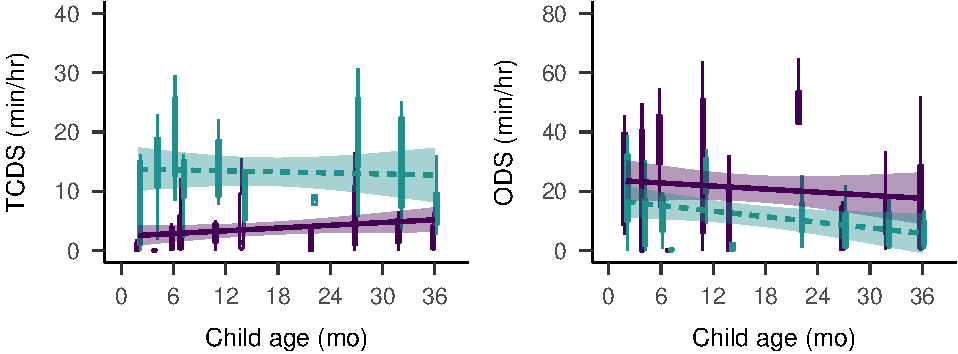
\includegraphics{Tseltal-CLE_files/figure-latex/fig1-1.pdf}
\caption{\label{fig:fig1}By-child estimates of minutes per hour of overheard
speech (left), target-child-directed speech (right). Data are shown for
the random (purple; solid) and turn taking (green; dashed) samples.
Bands on the solid linear trends show 95\% CIs.}
\end{figure}

\subsubsection{Target-child directed speech
(TCDS)}\label{target-child-directed-speech-tcds}

The Tseltal children in our study were directly spoken to for an average
of 3.63 minutes per hour in the random sample (median = 4.08; range =
0.83--6.55) and 13.28 minutes per hour in the turn-taking sample (median
= 13.65; range = 7.32--20.19).

The rate of TCDS was primarily affected by factors relating to the time
of day. The conditional model of randomly sampled clips showed that,
overall, children were more likely to hear TCDS in the mornings and
evenings than around midday (MODEL-REF). However, in both the randomly
sampled clips and the turn-taking clips, the conditional models showed
that this pattern weakened for older children, some of whom even heard
peak TCDS input around midday (\protect\hyperlink{fig2}{figure 2};
random: MODEL-REF; turn taking: MODEL-REF). There were no significant
effects of child age, household size, number of speakers present, or
maternal education in either model, and no significant effects in the
zero-inflation
models\footnote{The zero-inflation model for TCDS min/hr would not converge with time of day or number of speakers present.}.

\begin{figure}
\centering
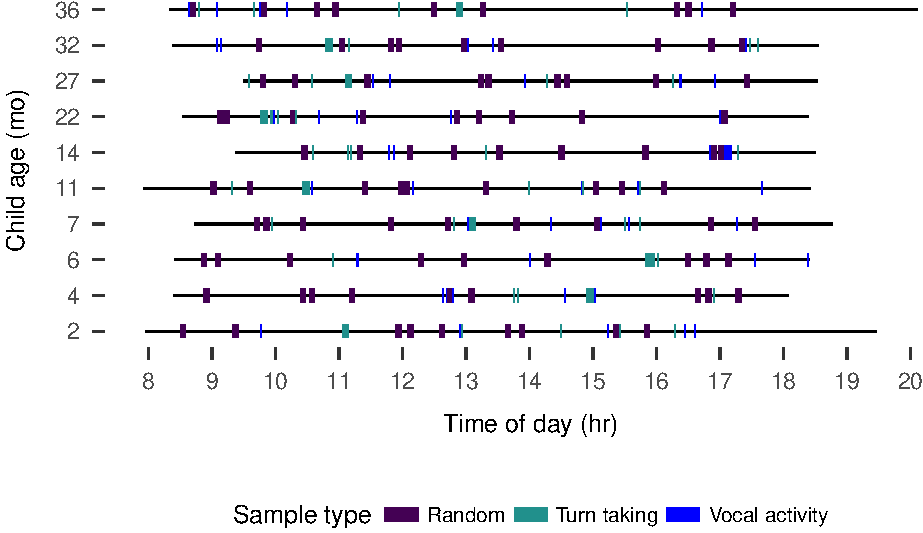
\includegraphics{Tseltal-CLE_files/figure-latex/fig2-1.pdf}
\caption{\label{fig:fig2}TCDS rate heard at different times of day by
children 12 months and younger (left) and 13 months and older (right) in
the randomly selected (purple) and turn-taking (green) clips.}
\end{figure}

\subsubsection{Other directed speech
(ODS)}\label{other-directed-speech-ods}

The children in our corpus frequently heard speech directed to others:
an average of 21.05 minutes per hour in the random sample (median =
17.80; range = 3.57--42.80) and 11.93 minutes per hour in the
turn-taking sample (median = 10.18; range = 1.37--24.42). That is, on
average during their daylong recording, children heard 5--6 times as
much speech directed to others than was directed to them. Even in the
period of maximal interaction, children heard nearly equal amounts of
speech directed to them and speech directed to others.

The conditional models of ODS revealed a that the presence of more
speakers was strongly associated with more ODS, in both the random
(MODEL-REF) and turn-taking (MODEL-REF) clips. Additionally, more ODS
occurred in the mornings and evenings (MODEL-REF), and was also more
frequent in large households for older children compared to younger
children (MODEL-REF). There were no other significant effects on ODS
rate in the conditional models, and no significant effects in the
zero-inflation
models\footnote{Neither zero-inflation model for ODS min/hr would converge with number of speakers present, and so only include time of day.}.

\subsection{Speaker environment}\label{speaker-environment}

As reviewed above, previous work on Mayan communities, including the
Tseltal community suggests that Mayan children hear much of their TCDS
from other children, and that the proportion of TCDS from other children
increases with age (REFS). North American infants (6--7 months) tend to
live in nuclear family homes but, during 16-hour daylong recordings,
often hear speech from four individuals during a short period (REFS;
cite\{bergelsonetal2018daybyday\}), and their developing ability to walk
away and self-entertain has been proposed as a hypothesis for decreasing
overheard speech with age (REFS; cite\{bergelsoncasillas2018\}). We
investigated whether these same patterns held up for the children in the
current corpus.

\subsubsection{Number of speakers}\label{number-of-speakers}

There were an average 3.44 speakers present other than the target child
in the randomly selected clips (median = 3; range = 0--10), and 2.56
non-target-child speakers present in the turn taking clips (median = 2;
range = 1--6). Children accounted for a little less than half of the
speakers present; the average number of child speakers in the randomly
selected clips was 1.44 (median = 2; range = 0--5) and in the turn
taking clips was 0.86 (median = 1; range = 0--4).

We modeled the number of speakers present in the randomly selected and
turn-taking clips using poisson linear regressions due to the fact that
the dependent variable is integer count data (REFS). Each model included
random slopes of chils and the age-related predictors of
interest---child age (standardized) and two-way interactions between
child age and household size (standardized) and child age and time of
day (centered on noon, squared, and then standardized). The fixed
effects also included household size and and time of day again as
nuisance variables.

There was no evidence of age-related change in the number of speakers
present. The total number of speakers was only significantly affeced by
the time of day in the random clips (MODEL-REF), and was not
significanly influenced by any of the predictors in the turn-taking
clips. We a second set of models, this time only analyzing the number of
child speakers present and found parallel results to the first set of
models (randomly selected clips: MODEL-REF; turn-taking clips: no
significant effects).

\subsubsection{Proportion TCDS from other
children}\label{proportion-tcds-from-other-children}

Most TCDS heard by the children in our corpus came from adults: on
average, only 19\% of TCDS came from child speakers. We used a binomial
model to evaluate whether the likelihood of hearing TCDS from a child in
a clip increased with age
(REF).\footnote{We were unable to run a beta regression on the proportion of TCDS with age given that most of the clip values were at or near 0 or 1; thereby motivating the binomial analysis reported here.}
We found no evidence that TCDS from other children increased with age in
the randomly sampled or turn-taking clips (MODEL-REF). We also performed
a Spearman's correlation between the child's age and the mean number of
child talkers, but neither showed a significant relationship
(MODEL-REFS).

\subsection{Interactional exchanges}\label{interactional-exchanges}

We can also measure children's linguistic environments as a summary of
the interactional exchanges they partake in (see also Romeo REFS). When
children are jointly engaged with an interlocutor, they can practice
making contingent vocalizations, and both the child and the interlocutor
can more easily coordinate their behaviors and social and communicative
intentions. In what follows, we characterize children's interactional
exchanges with four measures: the rate of child-to-other turn
transitions (i.e., contingent responses to the child's vocalizations),
the rate of other-to-child turn transitions (i.e., contingent responses
by the child), the duration of interactional turn-taking sequences
involving the target child, and the ratio of interlocutor vs.~child
vocalization time. We first describe these measures with respect to the
random sample then, for comparison, we examine the turn-taking sample.

\begin{figure}
\centering
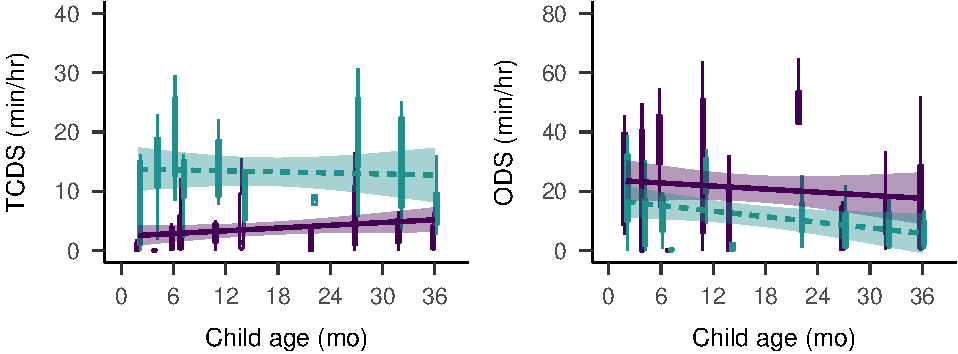
\includegraphics{Tseltal-CLE_files/figure-latex/fig3-1.pdf}
\caption{\label{fig:fig3}By-child estimates of contingent responses per
minute to the target child's vocalizations (upper left), contingent
responses per minute by the target child to others'
target-child-directed speech (upper right), the average duration of
contingent interactional sequences (lower left), and the ratio of
vocalization time between target children and target-child-directed
speech (lower right). Each datapoint represents the value for a single
clip within the random (purple; solid) or turn taking (green; dashed)
samples. Bands on the solid linear trends show 95\% CIs.}
\end{figure}

\subsubsection{Contingent response rate}\label{contingent-response-rate}

\subsubsection{Interactional sequences
duration}\label{interactional-sequences-duration}

\subsubsection{Vocalization ratio}\label{vocalization-ratio}

We detect contingent turn exchanges between the target child and other
speakers based on turn timing (). If there is a target-child-directed
utterance that begins between the start of a target child vocalization
and 2000msec after the end of the child's vocalization, we count it as a
CHI-OTH turn transition Similarly, if there is a target child
vocalization that begins between the start of a target-child-directed
utterance and 2000msec after the end of the utterance, it is counted as
a OTH-CHI turn transition. Each utterance is maximally allowed to act as
one prompt for a child vocalization and one response to a child
vocalization (e.g., in an CHI--OTH--CHI turn-taking sequence). We
identify sequences of interaction using a similar mechanism: we look for
chains of contingent responses before and after each child vocalization,
allowing for speakers to continue with multiple vocalizations/utterances
between speaker exchanges (). In this case, we also limit the overlap
between utterances because we are focused here on interactional exchange
that primarily features speech by one speaker at a time. Sequences are
bounded by the earliest and latest vocalization for which there is no
contingent prompt/response, respectively. Sequences must have at least
one contingent non-target-child utterance. Finally, each child
vocalization can only appear in one sequence, and many sequences have
more than one child vocalization.

We base these timing restrictions on vocal contingency on prior studyes
of infant and young children's turn taking. Hilbrink et al. (2015; REFS)
found that infants' (0;3--1;6) responses to mothers typically began
between -700ms and 1200ms relative to the end of the mothers' turns and
mothers' responses to their infants began between -350ms and 650ms
relative to the end of the infants' turns. Casillas et al. (2016; REFS)
found that children's responses to caregivers' questions typically
started between -500ms and 650ms relative to their caregiver's turn end,
and caregivers' responses to children's question between -1000ms and
400ms relative to the children's turn end. Because both studies focused
on fairly intensive bouts of interaction, and both within WEIRD parental
contexts, we defined contingent responses in the current data with more
generous allowances for overlap and gap (gap = 2000; overlap = 1000).
That said, our timing restrictions are much tighter than those used to
define interactional contingency in many other studies (e.g., REFS, see
also REFS for a review on adult-adult turn timing).

\subsection{Vocal maturity}\label{vocal-maturity}

\subsubsection{Developmental trajectory}\label{developmental-trajectory}

\subsubsection{Relation to language
experience}\label{relation-to-language-experience}

\section{Discussion}\label{disc}

\subsection{Future directions}\label{disc-future}

\subsection{Conclusion}\label{disc-conclusion}

\section{Acknowledgements}\label{acknowledgements}

\newpage

\section{References}\label{refs}

\begingroup
\setlength{\parindent}{-0.5in} \setlength{\leftskip}{0.5in}

\hypertarget{refs}{}

\endgroup






\end{document}
